\begin{frame}[fragile]{Fusión de ramas}
    \begin{columns}
      \column{0.48\textwidth}
        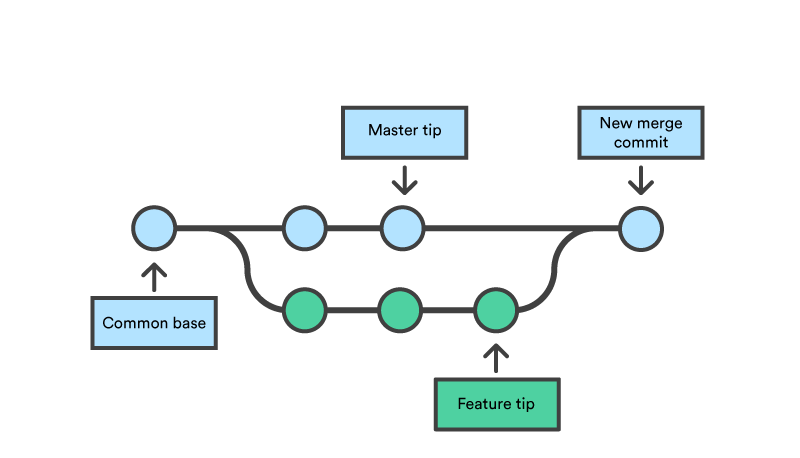
\includegraphics[scale=0.27]{images/branch-bitbucket}
      \column{0.52\textwidth}
      Si queremos fusionar dos ramas, nos posicionamos en la rama donde queremos que se apliquen los cambios y ejecutamos:
      \mint{console}| $ git merge <rama-a-fusionar>|
    \end{columns}
\end{frame}

\begin{frame}[fragile]{Fusión de ramas - \textsc{Fast-Forward}}
    \begin{columns}[onlytextwidth]
      \column{0.52\textwidth}
      \begin{exampleblock}{Ejemplo \textsc{Fast-Forward}:}
        \uncover<2->{
        \mint{console}| $ git checkout master|}
        \uncover<3->{
        \mint{console}| $ git merge hotfix|
        {\scriptsize \hspace{0.5cm} Adelanta el puntero de \texttt{master} a \texttt{hotfix}}}
        \uncover<4->{
        \mint{console}| $ git branch -d hotfix|}
      \end{exampleblock}
      \column{0.48\textwidth}
        \begin{figure}
          \only<1>{\scalebox{.95}{ \begin{tikzpicture}
  \gitDAG[grow right sep = 1.5em]{
    A -- B -- C -- {
    E,
    D},
  };
  \gitbranch
    {master}      % node name and text
    {above=of C} % node placement
    {C}          % target
  \gitbranch
    {issue53}      % node name and text
    {below=of D} % node placement
    {D}          % target
  \gitbranch
    {hotfix}      % node name and text
    {above=of E} % node placement
    {E}          % target
  % HDAD reference
  \gitHEAD
    {above=of hotfix} % node placement
    {hotfix}          % target
\end{tikzpicture}
}}
          \only<2>{\scalebox{.95}{ \begin{tikzpicture}
  \gitDAG[grow right sep = 1.5em]{
    A -- B -- C -- {
    E,
    D},
  };
  \gitbranch
    {master}      % node name and text
    {above=of C} % node placement
    {C}          % target
  \gitbranch
    {issue53}      % node name and text
    {below=of D} % node placement
    {D}          % target
  \gitbranch
    {hotfix}      % node name and text
    {above=of E} % node placement
    {E}          % target
  % HEAD reference
  \gitHEAD
    {above=of master} % node placement
    {master}          % target
\end{tikzpicture}
}}
          \only<3>{\scalebox{.95}{ \begin{tikzpicture}
  \gitDAG[grow right sep = 1.5em]{
    A -- B -- C -- {
    E,
    D},
  };
  \gitbranch
    {master}      % node name and text
    {above=of hotfix} % node placement
    {hotfix}          % target
  \gitbranch
    {issue53}      % node name and text
    {below=of D} % node placement
    {D}          % target
  \gitbranch
    {hotfix}      % node name and text
    {above=of E} % node placement
    {E}          % target
  % HEAD reference
  \gitHEAD
    {left=of master} % node placement
    {master}          % target
\end{tikzpicture}
}}
          \only<4>{\scalebox{.95}{ \begin{tikzpicture}
  \gitDAG[grow right sep = 1.5em]{
    A -- B -- C -- {
    E,
    D},
  };
  \gitbranch
    {master}      % node name and text
    {above=of E} % node placement
    {E}          % target
  \gitbranch
    {issue53}      % node name and text
    {below=of D} % node placement
    {D}          % target
  % HEAD reference
  \gitHEAD
    {above=of master} % node placement
    {master}          % target
\end{tikzpicture}
}}
        \end{figure}
    \end{columns}
\end{frame}

\begin{frame}[fragile]{Fusión de ramas - \textsc{3-way}}
    \begin{columns}[onlytextwidth]
      \column{0.52\textwidth}
      \begin{exampleblock}{Ejemplo \textsc{3-way}:}
        \uncover<2->{
        \mint{console}| $ git checkout master|}
        \uncover<3->{
        \mint{console}| $ git merge issue53|
        {\scriptsize \hspace{0.5cm} Crea un nuevo commit con la fusión a tres bandas de \\ \hspace{0.5cm} \texttt{master}, \texttt{issue53} y el \textbf{ancestro común} a ambas.}}
        \uncover<4->{
        \mint{console}| $ git branch -d issue53|}
      \end{exampleblock}
      \column{0.48\textwidth}
        \begin{figure}
          \only<1>{\scalebox{.85}{ \begin{tikzpicture}
  \gitDAG[grow right sep = 1.5em]{
    A -- B -- C -- {
    E -- G,
    D -- F},
  };
  \gitbranch
    {master}      % node name and text
    {above=of G} % node placement
    {G}          % target
  \gitbranch
    {issue53}      % node name and text
    {below=of F} % node placement
    {F}          % target
  % HEAD reference
  \gitHEAD
    {below=of issue53} % node placement
    {issue53}          % target
\end{tikzpicture}
}}
          \only<2>{\scalebox{.85}{ \begin{tikzpicture}
  \gitDAG[grow right sep = 1.5em]{
    A -- B -- C -- {
    E -- G,
    D -- F},
  };
  \gitbranch
    {master}      % node name and text
    {above=of G} % node placement
    {G}          % target
  \gitbranch
    {issue53}      % node name and text
    {below=of F} % node placement
    {F}          % target
  % HEAD reference
  \gitHEAD
    {above=of master} % node placement
    {master}          % target
\end{tikzpicture}
}}
          \only<3>{\scalebox{.80}{ \begin{tikzpicture}
  \gitDAG[grow right sep = 1.5em]{
    A -- B -- {[nodes=highlighted commit] {C}} -- {
      E -- {[nodes=highlighted commit] {G}} -- H,
      D -- {[nodes=highlighted commit] {F}} -- H},
  };
  \gitbranch
    {master}      % node name and text
    {above=of H} % node placement
    {H}          % target
  \gitbranch
    {issue53}      % node name and text
    {below=of F} % node placement
    {F}          % target
  % HEAD reference
  \gitHEAD
    {above=of master} % node placement
    {master}          % target
\end{tikzpicture}
}}
          \only<4>{\scalebox{.80}{ \begin{tikzpicture}
  \gitDAG[grow right sep = 1.5em]{
    A -- B -- C -- {
    E -- G -- H,
    D -- F -- H},
  };
  \gitbranch
    {master}      % node name and text
    {above=of H} % node placement
    {H}          % target
  % HEAD reference
  \gitHEAD
    {above=of master} % node placement
    {master}          % target
\end{tikzpicture}
} \\ \vspace{1.45cm}}
        \end{figure}
    \end{columns}
\end{frame}
